\section{Implementierung}
\label{Kapitel:Implementierung}
Zur Lösung der Strömungsgleichungen wurde die Programmbibliothek \linebreak \openfoam{} \cite{openfoam} verwendet.
%Diese wurde um die Implementierung der zugrunde liegenden Gleichungen und ihre Diskretisierung erweitert.
\openfoam{} ist eine freie CFD Bibliothek für Finite Volumen, in der zahlreiche Standardlöser schon implementiert sind.
Die Bibliothek erlaubt es auf komfortable Weise, eigenen Code zu implementieren.

Im Rahmen dieser Arbeit wurden die Modelle \eqref{eq:fg:carreauyasuda}, \eqref{eq:modHB} und \eqref{eq:whiteMetznerModell} als Erweiterung für schon vorhandene Löser eingebunden. Zusätzlich wurden eigene Konvergenzkriterien ausgewählt und die nötigen Auswertungsfunktionen implementiert.
Für die Simulation der viskoelastischen Fluide wurde als Basis ein Code von J.~Favero \cite{faveroOF} verwendet und an die in dieser Arbeit verwendeten Modelle und Gleichungen angepasst.
Dieses Kapitel gibt eine Übersicht über die verwendeten Methoden und Parameter, die Details der Implementierung stehen in Anhang~\ref{Kapitel:AnhangOpenFOAM}.

\subsection{Rheologische Modelle}
Die Implementierung der rheologischen Modelle geschah in Form von Bi\-blio\-the\-ken, die in \openfoam{} eingebaut werden können.

Ein Problem des verwendeten Herschel-Bulkley Modells \eqref{eq:modHB} ist der nicht definierte Wert der Viskosität bei $\gammap=0$.
Das Fluid sollte sich ohne Scherung theoretisch wie ein Festkörper verhalten und besitzt deshalb keine definierte Null-Viskosität (Abbildung~\ref{fig:hbclamp}).
Ein Strömungslöser wie \openfoam{} kann aber nicht ohne Weiteres den Übergang zwischen Festkörper und Fluid beschreiben. Deshalb wurde in der vorliegenden Arbeit die Viskosität nach oben beschränkt, so dass
%
\begin{equation}
    \eta = \min \left[ \eta_0,~\frac{\tau_0\cdot\left(1-\exp\left( -m\cdot\gammap \right)\right)+K\cdot \gammap^n}{\gammap} \right]
\end{equation}
%
gilt.
Diese Begrenzung ergänzt das Modell um eine Null-Viskosität und stabilisiert das Problem numerisch. Der Parameter $\eta_0$ kann dabei vom Benutzer festgelegt werden. Er sollte hoch genug gewählt werden, damit diese Viskositätsgrenze das Resultat der Simulation nicht beeinflusst. Eine zu hohe Grenze beeinflusst das Konvergenzverhalten aber negativ. Daher kann sie auch nicht beliebig hoch angesetzt werden.

Für die berechneten Fluide muss der Fliessindex $n$ stets kleiner als 1 gewählt werden, da die Mörtel strukturviskose Fluide sind.
Für $n<1$ gilt $\eta\rightarrow0$ für $\gammap\rightarrow\infty$. Diese Eigenschaft ist physikalisch nicht sinnvoll, da ein Fluid nicht unendlich flüssig werden kann. Deshalb wird die Viskosität $\eta$ nicht nur nach oben beschränkt, sondern auch nach unten.
Es wird für sehr hohe Scherraten eine minimale Viskostät $\eta_\infty$ eingeführt:
%
\begin{equation}
    \eta = \max \left[ \eta_\infty,~\min \left[ \eta_0,~\frac{\tau_0\cdot\left(1-\exp\left( -m\cdot\gammap \right)\right)+K\cdot \gammap^n}{\gammap} \right]\right].
\end{equation}
%

In der vorliegenden Arbeit wurden diese Werte auf eine Viskosität von $\eta_0=\SI{1.5e6}{Pa\,s}$ und $\eta_\infty=\SI{0.25}{Pa\,s}$ gesetzt.
Diese Grenzen wurden sowohl für die rein scherratenabhängigen als auch für die viskoelastischen Simulationen verwendet.
%
\begin{figure}
    \centering
    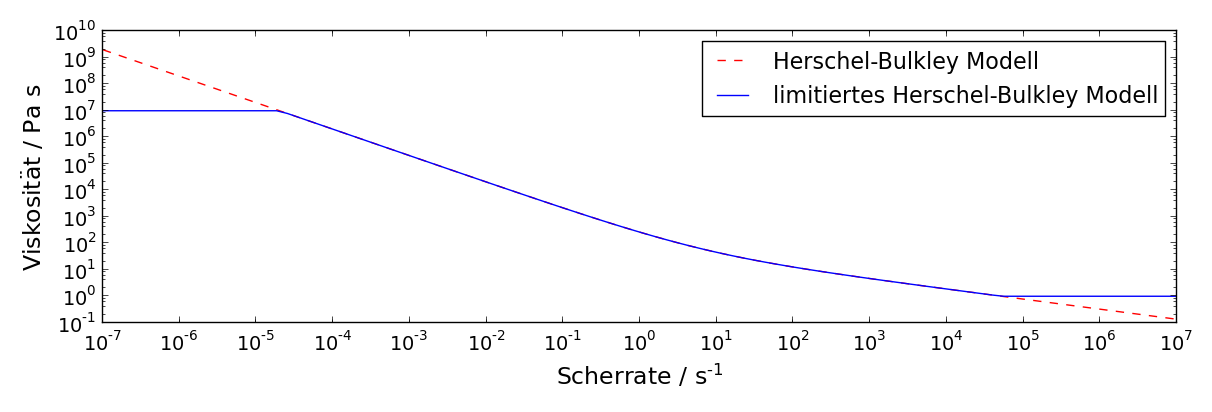
\includegraphics[width=\textwidth]{figures/hbclamp.png}
    \caption{Einfluss der Viskositätsbeschränkung auf das Herschel-Bulkley Modell. Die rote Linie zeigt das originale Modell, bei dem die Viskosität mit sinkender Scherrate ins Unendliche steigt (Festkörper). Die blaue Linie zeigt das limitierte Modell, dessen Viskosität sowohl nach oben als auch nach unten beschränkt ist.}
    \label{fig:hbclamp}
\end{figure}
%
\subsection{Löser}
Die Implementierung der in Kapitel \ref{Kapitel:Numerik} beschriebenen numerischen Verfahren SIMPLE und PISO ist in \openfoam{} weitgehend schon vorhanden.
Besondere Aufmerksamkeit muss aber der sich ändernden Viskosität ge"-schenkt werden. Diese bringt eine zusätzliche Nichtlinearität in die Impulserhaltungsgleichung ein und beeinflusst dadurch stark das Konvergenzverhalten. Zusätzlich hat sie für strukturviskose Fluide noch selbstverstärkende Effekte. In Regionen mit hoher Scherung liegt eine niedrige Viskosität vor, dadurch sind die Fliessgeschwindigkeiten höher und das Fluid wird noch mehr geschert. Hierdurch können in der numerischen Simulation schnell starke Schwingungen angefacht werden, die die Berechnung instabil ma\-chen.
Abbildung~\ref{fig:oszPress} zeigt solch eine Schwingung für eine Simulation. Hier ist der Druckverlauf am Einlass des in Kapitel \ref{Kapitel:Parameter} beschriebenen Kapillarrheometers gegen die als Iterationsindex verwendete Zeit aufgetragen.
%
\begin{figure}
    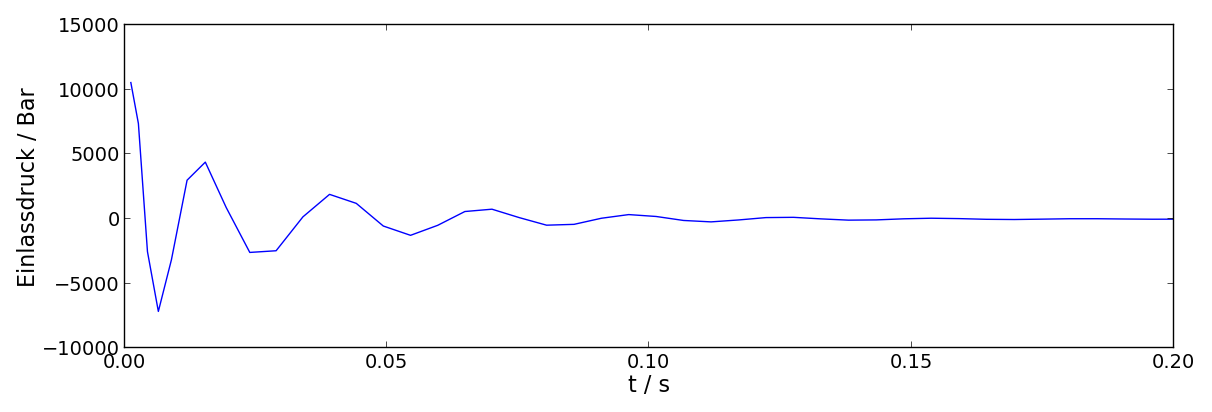
\includegraphics[width=\textwidth]{figures/schwankenderDruck.png}
    \caption{Einlassdruck eines Kapillarrheometers. Die scherratenabhängige Viskosität führt zu starken Oszillationen in der stationären Rechnung, die erst mit der Zeit verschwinden.}
    \label{fig:oszPress}
\end{figure}
%
Um diese Schwingungen zu dämpfen, wurde in stationären Berechnungen eine sehr starke Relaxation angewandt. Diese können in \openfoam{} für jedes berechnete Feld separat angegeben werden. Für den Druck $p$ wurden sie im Bereich von \num{3e-1} bis \num{1e-6}, für das Geschwindigkeitsfeld $\u$ zwischen \num{1e-1} und \num{1e-4} gewählt.

In transienten Simulationen kann keine Relaxation angewendet werden. Um die Stabilität der Rechnung trotzdem sicherzustellen, müssen sehr klei\-ne Zeitschritte gewählt werden.
%
\subsection{Konvergenzkriterien}
Die für Simulationen normalerweise verwendeten Residuen des Druck- und Geschwindigkeitsfeldes können in Berechnungen mit variabler Viskosität nicht ohne weiteres als Konvergenzkriterium verwendet werden.
Die Kopp\-lung von Geschwindigkeit und Viskosität führt dazu, dass die Lösung sich teilweise nur noch in kleinen Regionen um kleine Beträge ändert, diese Änderung sich aber durchaus noch über eine grosse Anzahl von Schritten fortsetzen kann. Dieser Effekt ist in Abbildung~\ref{fig:platRheoNu} verdeutlicht.
\begin{figure}
    \centering
    \subfloat[Viskosität nach 600 Schritten]{
    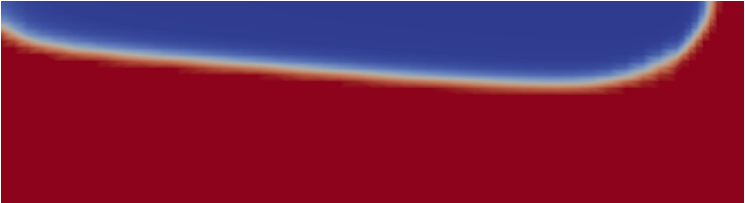
\includegraphics[width=0.45\textwidth]{figures/platRheoNu1.PNG}
    \label{fig:platRheoNu:subA}
    }
    \subfloat[Viskosität nach 10000 Schritten]{
    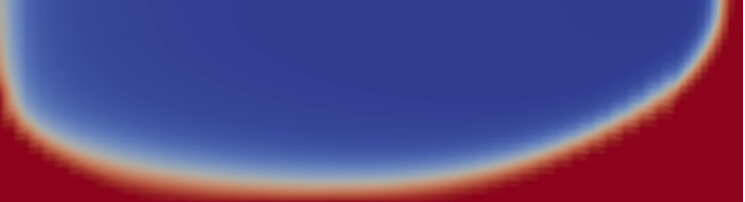
\includegraphics[width=0.45\textwidth]{figures/platRheoNu2.PNG}
    \label{fig:platRheoNu:subB}
    }
    \caption{Die Viskositätsverteilung (blau: niedrig, rot: hoch) im Platte-Platte Rheometer (Kapitel~\ref{Kapitel:Rheometer}) mit $\omega=\SI{10}{rad.s^{-1}}$ zu unterschiedlichen Zeitpunkten. Bereits nach 600 Schritten ist die Änderung zwischen zwei Schritten sehr klein, da die Viskosität sich nur noch unmittelbar an der in \subref{fig:platRheoNu:subA} zu sehenden Grenze ändert. Trotzdem unterscheidet sich das konvergierte Resultat in \subref{fig:platRheoNu:subB} deutlich von der noch nicht konvergierten Lösung.}
    \label{fig:platRheoNu}
\end{figure}
Daher wurde in der vorliegenden Arbeit statt der Residuen das Verhalten der aus den verwendeten Randbedingungen resultierenden Be"-ob"-ach"-tungs"-grös"-sen als Konvergenzkriterium verwendet.

Bei Simulationen mit einem am Einlass vorgegebenen Volumenstrom, wie beim Kapillarrheometer, ist dies der sich am Einlass einstellende Durchschnittsdruck:
%
\begin{equation}
    \overline p:= \frac{1}{A}\int_{x\in A}p\left( x \right).
\end{equation}
%

Für das Platte-Platte Rheometer ist die beobachtete Grösse nicht der Druck, sondern das resultierende Drehmoment.
Um dieses aus den berechneten Grössen zu ermitteln wird an den vom Nutzer bestimmten Flächen $A_i$ über die Schubspannung integriert:
%
\begin{equation}
    M = \sum_i \int_{A_i}r\cdot\tau\left( r \right)dA_i.
\end{equation}
Dabei ist
\begin{equation}
    \tau\left( r \right) = \eta\left( r \right) \cdot \frac{\partial \u\left( r \right)}{\partial \n\left( r \right)}
\end{equation}
die Schubspannung an der Wand und $r$ der Abstand zum Rotationszentrum.
Die Auswertung dieser Werte erfolgt in jedem Iterationsschritt. Die Änderung zwischen zwei Iterationsschritten kann dann als Konvergenzkriterium verwendet werden.
In Kapitel \ref{Kapitel:Parameter:PlattePlatteRheo} wird beschrieben wie die Viskosität des Mörtels anhand des Drehmomentes in einem Platte-Platte Rheometer bestimmt wird. 


Werden die Änderungen von Beobachtungsgrössen als Konvergenzkriterium verwendet, muss darauf geachtet werden, dass nicht nur die erste, sondern auch die zweite Ableitung mit einbezogen wird. Andernfalls ist es möglich, dass die Simulation zu früh gestoppt wird. Falls die beobachteten Werte zu Beginn der Simulation hin und her schwingen, nimmt die erste Ableitung in den Maxima und Minima ebenfalls sehr kleine Werte an, obwohl noch keine Konvergenz erreicht ist.
Die Ableitungen der beobachteten Werte wurden in dieser Arbeit mittels Finiten Differenzen berechnet:
%%
\begin{eqnarray}
    \label{eq:torqueCalc:fd}
    \dot{x} & = & \frac{1}{2}\left(  x[t+1] - x[t-1] \right), \\
    \ddot{x} & = & \frac{1}{2}\left(  x[t+1] - 2 \cdot x[t] + x[t-1] \right).
\end{eqnarray}
%
\subsection{Betriebssystem und Hardware}
\label{Kapitel:Hardware}
\openfoam{} kann nicht, beziehungsweise nur mit grossem Aufwand, auf Windows installiert werden. Einer der Gründe für diese Einschränkung ist, dass es eine Unterscheidung zwischen Gross- und Kleinschreibung bei Dateinamen benötigt. Die in dieser Arbeit verwendeten Betriebssysteme sind deshalb Linux"~Dis"-tri"-bu"-ti"-o"-nen.

Für kleinere lokale Berechnungen und Testläufe stand ein Laptop zur Verfügung, auf dem Ubuntu 12.04 LTS installiert wurde.
Der Hauptteil der Si"-mu"-la"-ti"-o"-nen wurde aber auf den HPC-Clustern des Swiss National Supercomputing Centre (CSCS) durchgeführt.
Mit dem im Tessin gelegenen Cluster \emph{Rothorn} stand ein Berechnungsknoten mit 256 CPUs zur Verfügung. Das System ist ein SGI Altix UV 1000, das für Berechnungen einen Ar"-beits"-spei"-cher von 2TB besitzt.
Das Betriebssystem ist SUSE SLES11 SP1.
Der Zugang zum Cluster erfolgt über eine 'secure shell' (ssh) Verbindung, mit der man sich über den Zugangsknoten \emph{Ela} auf \emph{Rothorn} einloggen kann.

Die visuelle Nachbearbeitung der Resultate wurde ebenfalls auf Rech\-nern des CSCS durchgeführt. Allerdings nicht auf \emph{Rothorn} sondern auf dem \linebreak Dalco SM System \emph{Eiger}.
Zur Visualisierung wird eine graphische Benutzer"-oberfläche benötigt. Die 'secure shell' Methode ist hierfür nicht geeignet, da damit nur eine Konsole auf dem entfernten Rechner geöffnet werden kann. Deshalb erfolgte der Zugang auf \emph{Eiger} über eine 'virtual network compu\-ting' (vnc) Verbindung. Hierbei wird die Bildschirmausgabe des entfernten Computers auf eine lokale Maschine übertragen und im Gegenzug Maus- und Tastatureingaben zurück gesendet.

Diese Art der Auslagerung von Rechnungen auf einen Cluster ermöglicht es, auch grosse und zeitaufwändige Simulationen von einem lokalen Computer aus zu starten und auszuwerten, ohne dass grosse Mengen an Daten hin und her kopiert werden müssen.
